%% Dit is de domeinanalyse: Combinatorial Objects %%
%% Freek 26 september: Een derde domeinanalyse zou kunnen gaan over hoe om te
%% gaan met combinatorial objects (bijv. hoe grafisch weer te geven, hoe op te
%% slaan in de data structuur)

\documentclass[a4paper,11pt,final]{article}

\usepackage[english]{babel}
\usepackage{graphicx}
\usepackage{hyperref}
\hypersetup{ colorlinks = true, citecolor = blue,linkcolor = blue }
\usepackage[a4paper]{geometry}
\usepackage{titlesec}% added to change section headers, see newcommand definition.


\bibliographystyle{alpha}

		

\begin{document}
\selectlanguage{english}
\begin{titlepage}
	\vspace*{\fill}
	\begin{center}
		\textsc{\large WickedXmas Domain Analysis}\\[0.5cm]
		\textsc{\huge Combinatorial Objects}\\[0.5cm]
		\textsc{Stefan Versluys}\\ \textsc{\scriptsize 19/10/2014}\\[2.0cm]
		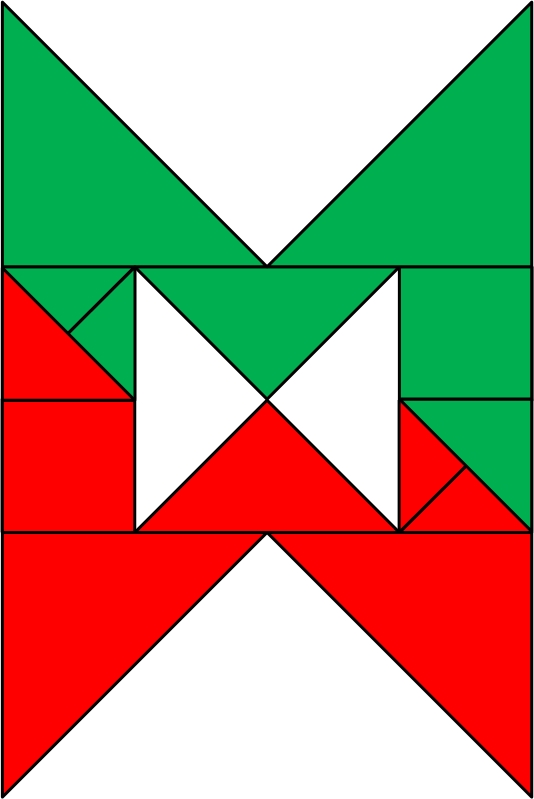
\includegraphics[width=0.25\textwidth]{wXm}
	\end{center}
	\vspace*{\fill}
\end{titlepage}


\tableofcontents

\newpage

\section{Introduction}
This domain analysis concerns combinatorial objects,
along with primitive objects this kind of objects can be used to design xMAS
models with the WickedXmas tool. In fact combinatorial objects are xMAS models
itself but left open with unconnected ports, parameterizable and allow recursive reuse.

The benefits of combinatorial objects are those of reusability, it makes complex things look simple and maintainable, it preserves correctness.

When designing an xMAS model in WickedXmas , the designer can make use of combinatorial objects similar as he or she does with primitive objects. Because
combinatorial objects are xMAS models these can be edited just as any other kind of xMAS model except that there are unconnected ports as mentioned before.


\section{xMAS Modelling}
To visualise an xMAS model in the WickedXmas tool,
objects have graphical properties. To parametrize xMAS models, objects and the
models also have some specific properties. Properties and communication logic,
which control the message flow during verification, are not used during
modelling in the WickedXmas tool. 

In other words, this document only concerns
the properties necessary to represent an xMAS model so it can be visualized,
edited, stored and exchanged with the verification interface.
 

\newpage
\section{Primitive objects}
Primitive objects are the base of combinatorial objects and determine the underlying structures.
Secondly, when using objects to create a model, there are a lot of similarities between
combinatorial and primitive objects. With this knowledge we can say that
primitive objects need some explanation as far as these are concerned with
combinatorial objects and modelling using WickedXmas.

The xMAS language has only eight primitive objects,
each object has a visual representation and one or more properties which can be
changed by the user. Some of these properties requires a valid value otherwise a
visual marker, shown as a dot as part of the object, will lit up red instead of
green. Finally all objects have one or more ports and can be of input or output
type. The graphical representation of a port is a red filled square. Each port
must be wired to exactly one opposite porttype of an other object to form a valid
channel.

\paragraph{Common properties:}
\begin{itemize}
\item Label: A string which identifies the object.
\item Position: x and y-coordinates where the object is drawn on screen.
\item Orientation: A rotation value of how the object will be drawn on screen.
\end{itemize}

\subsection{Queue}
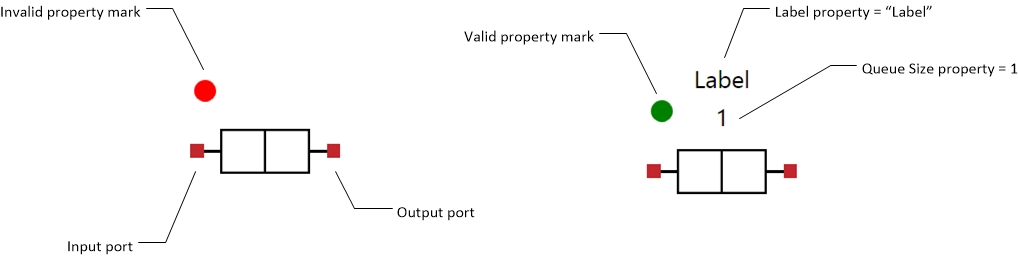
\includegraphics[width=1.0\textwidth]{queue}
The queue object its valid marker becomes green when the size property is a natural number $>$ 0. 
The queue also have a "state" property to show the verification result. 
\paragraph{Specific properties:}
\begin{itemize}
\item Size: A positive integer which represents the storage size of a queue.
\item State: A flag to show the verification result.
\end{itemize}

\subsection{Function}

\includegraphics[width=1.0\textwidth]{function}
\paragraph{Specific properties:}

\begin{itemize}
\item Function f: is a subset of the C language, an integer which represents the packet is available through variable 'header'. The valid marker becomes green if the  string value of the Function f property is not empty. Example: ret=0;

Available operators:
\begin{itemize}
\item math operators $+,-,*,/,\%$
\item logical operators $\&\&,||,!$
\item equality operators $==,<=,>=,<,>$
\end{itemize}
\end{itemize}


\subsection{Fork}
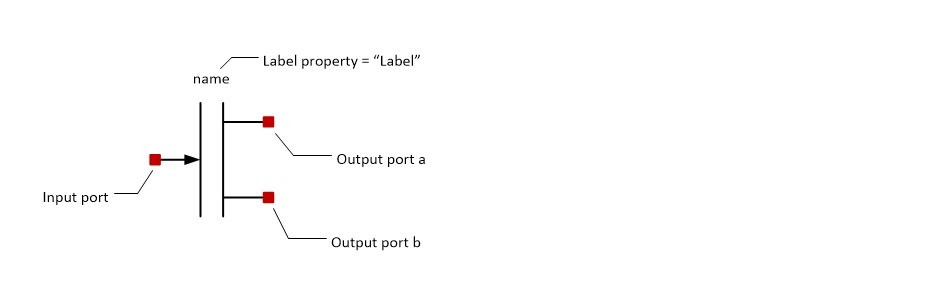
\includegraphics[width=1.0\textwidth]{fork}

A fork has no specific properties.

\subsection{Join}
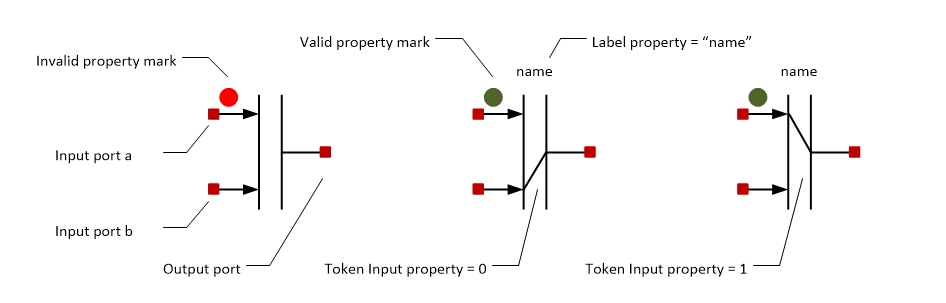
\includegraphics[width=1.0\textwidth]{join}

The join object its valid marker becomes green if the "token" property is set. Depending on the "token" property the visualisation of the object will change.
\paragraph{Specific properties:}
\begin{itemize}
\item Token Input: "0" select input 2 while "1" selects input 1
\end{itemize}



\subsection{Switch}
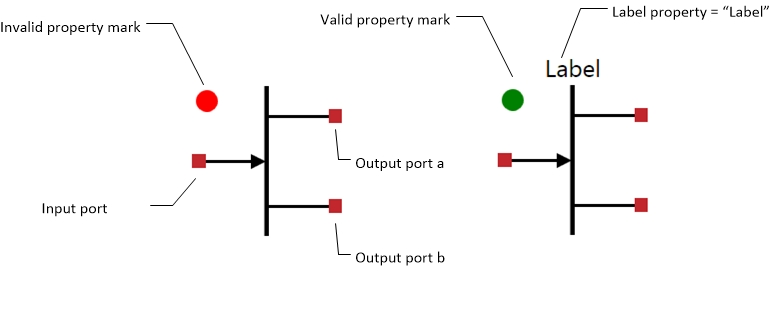
\includegraphics[width=1.0\textwidth]{switch}
Property "Function s" is a subset of the C language, an integer which represents the packet is available through variable 'header'.
\begin{itemize}
\item math operators $+,-,*,/,\%$
\item logical operators $\&\&,||,!$
\item equality operators $==,<=,>=,<,>$
\end{itemize}
Example function : return header == 0;
ToDo : description + fjson structure
\subsection{Merge}
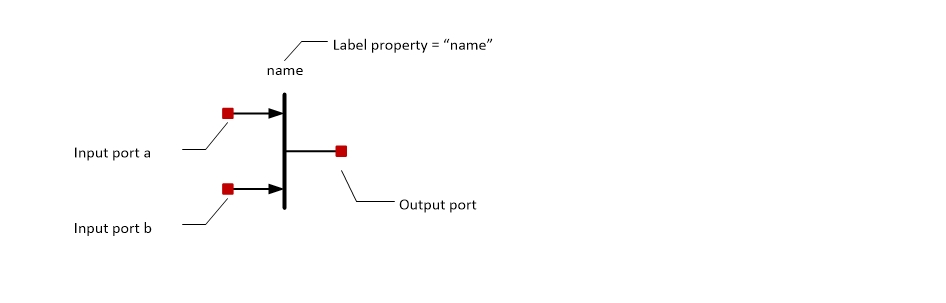
\includegraphics[width=1.0\textwidth]{merge}

ToDo : description + fjson structure

\subsection{Sink}
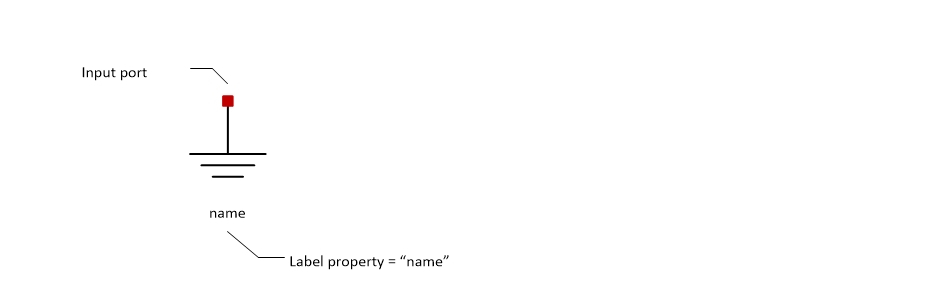
\includegraphics[width=1.0\textwidth]{sink}

ToDo : description + fjson structure

\subsection{Source}
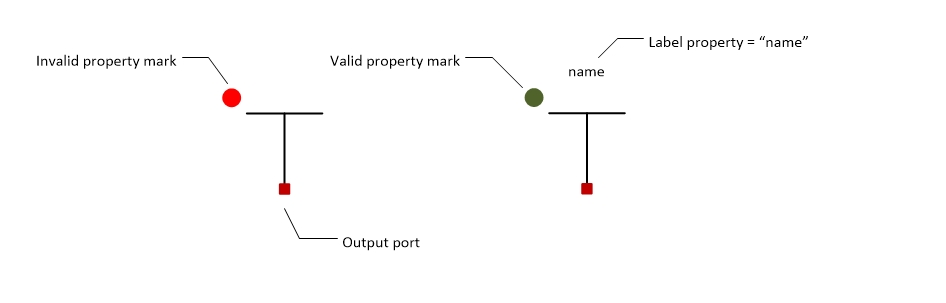
\includegraphics[width=1.0\textwidth]{source}

Property "Function e" insert types of packets injected at this source. The
domain of all packets is available through PacketDomain.

ToDo : description + fjson structure

\newpage
\section{Combinatorial objects} To create combinatorial objects, which
means an open network, we need something to distinguish between an dangling portor a port that can be connected later when re-using the combinatorial object.
Example : {p in PacketDomain | p < 100}

ToDo : to be completed
\subsection{Recursion}
\subsection{Macro}
\subsection{Visual representation}
\subsection{Structure}

\newpage
\section{JSON}
ToDo : to be completed
\subsection{Hierarchical structure}
\subsection{Flat structure}

\newpage
\section{Similar domain examples}
ToDo : example of how a similar product manages re-usable components

\newpage
\section{Dictionary}
\begin{itemize}
	\item \textbf{WickedXmas}: Name ofthe tool used to design and analyse xMAS models.
	\item \textbf{xMAS model}: A model based on Intel's xMAS or e\underline{x}ecutable \underline{M}icro\underline{A}rchitectural \underline{S}pecification, which is ahigh level design language for communication fabrics.
	\item \textbf{Primitive Object}: The xMAS language consist of eight primitive objects which are used to create xMAS models. Primitive objects are hard coded.
	\item \textbf{Combinatorial Object}: A composite object which can be made of primitives and combinatorial objects. It is also known as a open xMAS model or macro.
	\item \textbf{Channel}: A connection between an input and output port.
	\item \textbf{Port}: Each object has one or more ports to create a channel, there are initiator and target ports.
	\item \textbf{Initiator}: An output port.
	\item \textbf{Target}: An input port.
	\item \textbf{Open xMAS network}: see combinatorial object.
	\item \textbf{Macro or macro block}: see combinatorial object.
	\item \textbf{Configuration}: Represents the current state of a model which means the occupation of queues.
	\item \textbf{wck}: File extension of an xMAS model and contains hierarchical structured JSON.
	\item \textbf{JSON}: \underline{J}avascript \underline{O}bject \underline{N}otation is a readable data file format comparable to XML.
	\item \textbf{fjson}: File extension of an xMAS model and contains flat structured JSON.
	\item \textbf{Message type}: Thereresponse or request
\end{itemize}

\end{document}